\section{Identyfikacja charakterystyk statycznych}

Aby wykorzystać zaproponowany w rozdziale 1 model, trzeba wiedzieć jak zależą prędkości śmigieł od napięć sterujących oraz jak siła ciągu śmigieł zależy od ich prędkości obrotu. W tym celu należy wyznaczyć charakterystyki statyczne $\omega_m(U_m), \omega_t(U_t), F_m(\omega_m)$ i $F_t(\omega_t)$

\subsection{Zależność prędkości śmigieł od napięcia}

Zbadanie zależności $\omega_m(U_m)$ i $\omega_t(U_t)$ polegało na przeprowadzeniu eksperymentu przedstawionego na wykresie \ref{rys:pr_silniki}. Podczas trwającego 240 sekund doświadczenia liniowo zmieniano napięcie zasilające silniki przy śmigłach i mierzono prędkość wyjściową z użyciem tachoprądnicy. Powoli zmieniające się sterowanie pozwalało na obserwację prędkości silników w przybliżeniu "ustalonej" po każdej niewielkiej zmianie.

Założono, że tachoprądnica wskazuje zmianę napięcia o 0.52V na każde 1000 rpm zmiany prędkości obrotowej, zgodnie z dokumentacją.% \ref{tacho}.
% http://aq.ia.agh.edu.pl/Aquarium/Dydaktyk/Laborat/LP/Tacho_tras.pdf

\begin{figure}[!htb]
\centering
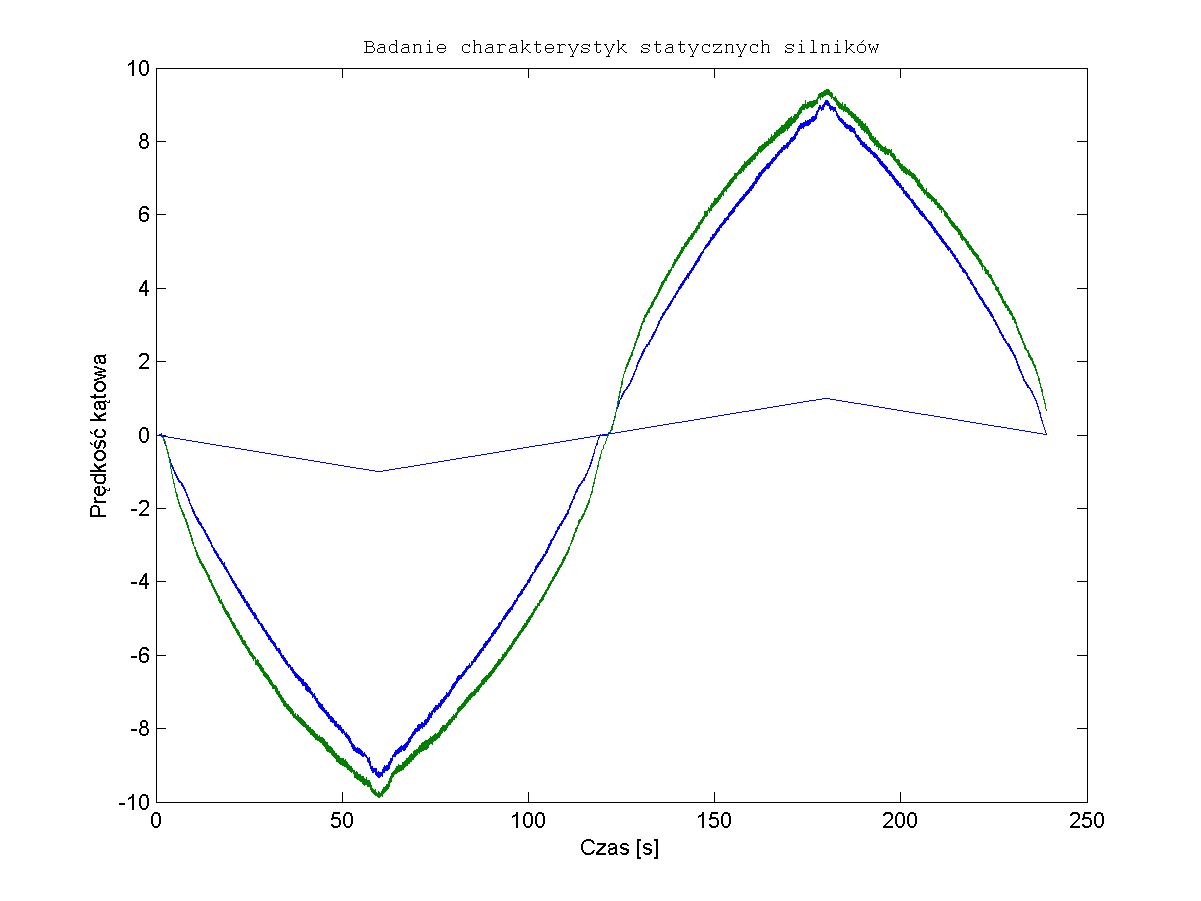
\includegraphics[scale=0.85]{img/predkosc_silniki.png}
\caption{Eksperyment wyznaczenia charakterystyk prędkości od napięcia przy zablokowanych osiach}
\label{rys:pr_silniki}
\end{figure}

Charakterystyki prędkości w funkcji sterowania przedstawia wykres \ref{rys:char_omega}. 
Na wykresie widoczna jest histereza, większa w przypadku śmigła tylnego. Oznacza to, że śmigło ma inną prędkość dla tego samego napięcia zależnie od tego, czy właśnie się rozpędza, czy zwalnia.

\begin{figure}[!htb]
\centering
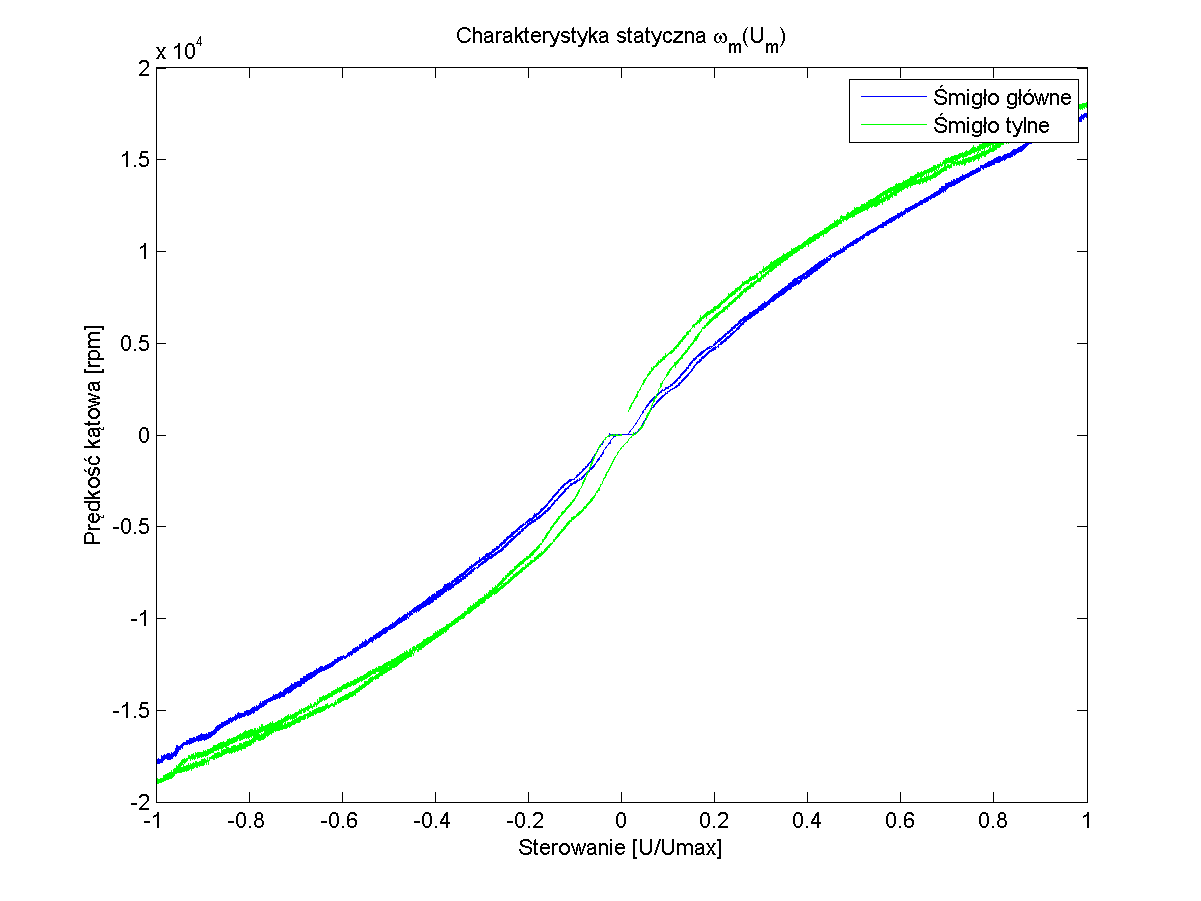
\includegraphics[scale=0.85]{img/char_stat_omega.png}
\caption{Eksperyment wyznaczenia charakterystyk prędkości od napięcia przy zablokowanych osiach}
\label{rys:char_omega}
\end{figure}

\subsection{Oszacowanie wpływu tarcia na układ}

\begin{figure}[!htb]
\centering
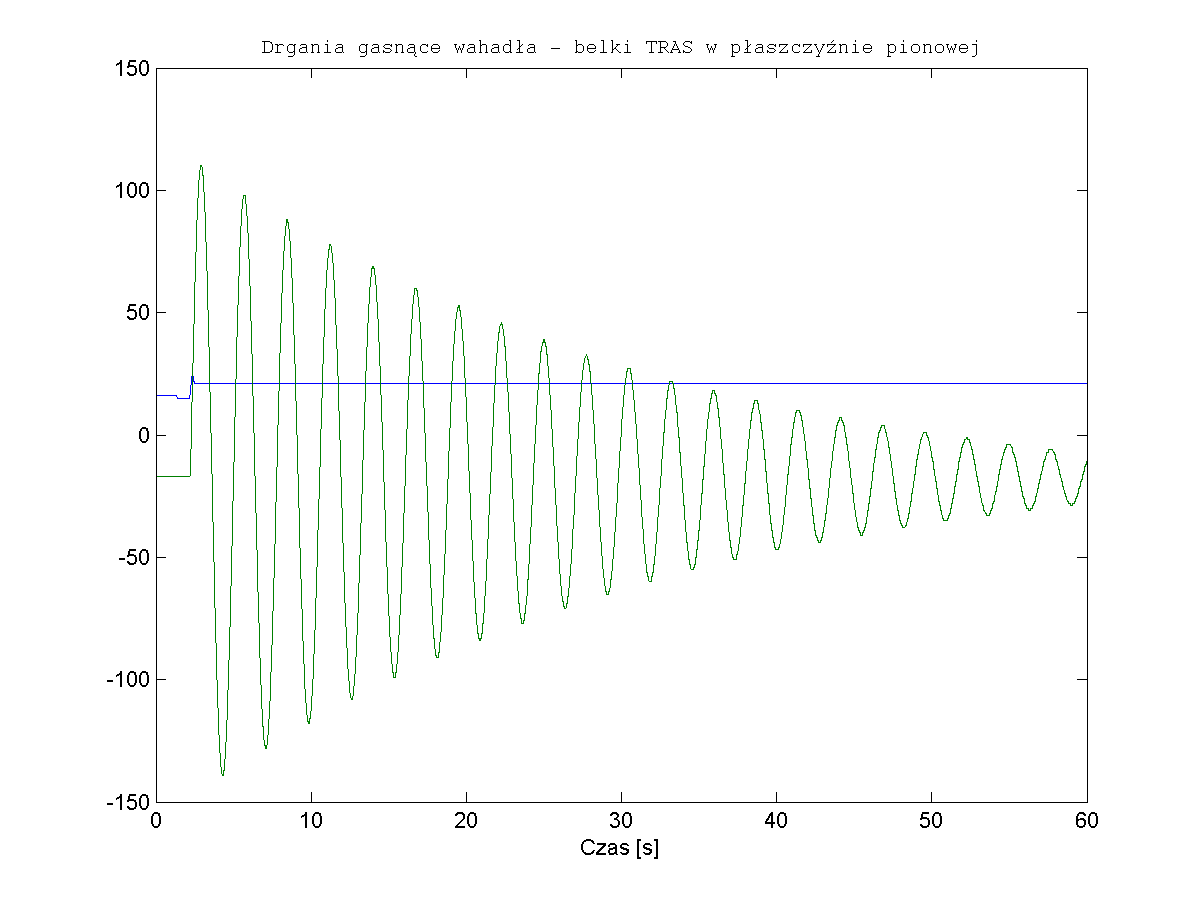
\includegraphics[scale=0.85]{img/gasnace.png}
\caption{Identyfikacja oporów tarcia belki w płaszczyźnie pionowej}
\label{rys:gasnace}
\end{figure}


